\documentclass[sigconf]{acmart}

\usepackage{listings}
\usepackage{color}
% \usepackage[parfill]{parskip}

\definecolor{dkgreen}{rgb}{0,0.6,0}
\definecolor{gray}{rgb}{0.5,0.5,0.5}
\definecolor{mauve}{rgb}{0.58,0,0.82}

\lstset{frame=tb,
  language=Python,
  aboveskip=3mm,
  belowskip=3mm,
  showstringspaces=false,
  columns=flexible,
  basicstyle={\small\ttfamily},
  numbers=none,
  numberstyle=\tiny\color{gray},
  keywordstyle=\color{blue},
  commentstyle=\color{dkgreen},
  stringstyle=\color{mauve},
  breaklines=true,
  breakatwhitespace=true
  tabsize=3
}

\def\bZ{\mathbb{Z}}
\def\bN{\mathbb{N}}
\def\bR{\mathbb{R}}
\def\bC{\mathbb{C}}
\def\bQ{\mathbb{Q}}
\usepackage{hyperref}

\usepackage{endfloat}
\renewcommand{\efloatseparator}{\mbox{}} % no new page between figures

\usepackage{booktabs} % For formal tables

\settopmatter{printacmref=false} % Removes citation information below abstract
\renewcommand\footnotetextcopyrightpermission[1]{} % removes footnote with conference information in first column
\pagestyle{plain} % removes running headers
\usepackage{indentfirst}
 
\begin{document}
\title{Big Data analytics in predict house price}


\author{Yujie Wu}
\affiliation{%
  \institution{Indiana University Bloomington}
  \city{Bloomington} 
  \state{Indiana} 
  \postcode{47401}
}
\email{yujiwu@iu.edu}



% The default list of authors is too long for headers}
\renewcommand{\shortauthors}{B. Trovato et al.}


\begin{abstract}
\large  House price changes dynamically and it costs human power to evaluate the price. This project uses a large data set obtained from house dealings and algorithms to predict if house price is reasonable.
\end{abstract}

\keywords{\large i523, HID235, House Price, Logistic Regression, linear Regression}

\maketitle

\section{Introduction}
\large Asking a home buyer to describe their dream house, and they probably won't begin with the height of the basement ceiling or the proximity to an east-west railroad. But this playground competition's dataset proves that much more influences price negotiations than the number of bedrooms or a white-picket fence. With 79 explanatory variables describing (almost) every aspect of residential homes in Ames, Iowa, this project is aimed to overcome the challenges of predicting the final price of each home.

\section{Linear regression}
\par In statistics, linear regression is a linear approach for modeling the relationship between a scalar dependent variable y and one or more explanatory variables (or independent variables) denoted X. The case of one explanatory variable is called simple linear regression. For more than one explanatory variable, the process is called multiple linear regression.

In linear regression, the relationships are modeled using linear predictor functions whose unknown model parameters are estimated from the data. Such models are called linear models. Most commonly, the conditional mean of y given the value of X is assumed to be an affine function of X; less commonly, the median or some other quantile of the conditional distribution of y given X is expressed as a linear function of X. Like all forms of regression analysis, linear regression focuses on the conditional probability distribution of y given X, rather than on the joint probability distribution of y and X, which is the domain of multivariate analysis.

Linear regression was the first type of regression analysis to be studied rigorously, and to be used extensively in practical applications. This is because models which depend linearly on their unknown parameters are easier to fit than models which are non-linearly related to their parameters and because the statistical properties of the resulting estimators are easier to determine.

\section{Logistic regression}
\par In statistics, logistic regression, or logit regression, or logit model is a regression model where the dependent variable (DV) is categorical. This article covers the case of a binary dependent variable that is, where the output can take only two values, "0" and "1", which represent outcomes such as pass/fail, win/lose, alive/dead or healthy/sick. Cases where the dependent variable has more than two outcome categories may be analyzed in multinomial logistic regression, or, if the multiple categories are ordered, in ordinal logistic regression. In the terminology of economics, logistic regression is an example of a qualitative response/discrete choice model.

Logistic regression was developed by statistician David Cox in 1958. The binary logistic model is used to estimate the probability of a binary response based on one or more predictor (or independent) variables (features). It allows one to say that the presence of a risk factor increases the odds of a given outcome by a specific factor.

Logistic regression is used in various fields, including machine learning, most medical fields, and social sciences. For example, the Trauma and Injury Severity Score (TRISS), which is widely used to predict mortality in injured patients, was originally developed by Boyd et al. using logistic regression. Many other medical scales used to assess severity of a patient have been developed using logistic regression. Logistic regression may be used to predict whether a patient has a given disease (e.g. diabetes; coronary heart disease), based on observed characteristics of the patient. Another example might be to predict whether an American voter will vote Democratic or Republican, based on age, income, sex, race, state of residence, votes in previous elections, etc. The technique can also be used in engineering, especially for predicting the probability of failure of a given process, system or product.It is also used in marketing applications such as prediction of a customer's propensity to purchase a product or halt a subscription, etc. In economics it can be used to predict the likelihood of a person's choosing to be in the labor force, and a business application would be to predict the likelihood of a homeowner defaulting on a mortgage. Conditional random fields, an extension of logistic regression to sequential data, are used in natural language processing.


\section{Experiment}
\begin{lstlisting}
In [1]: import matplotlib.pyplot as plt
        % matplotlib inline
        from sklearn.metrics import accuracy_score
In [2]: from sklearn.ensemble import RandomForestClassifier
        import pandas as pd
        from sklearn.preprocessing import LabelEncoder
        import numpy as np
        df=pd.read_csv('C:\\Users\\Yujie\'s
        VMware\\Desktop\\training_data.csv')
        df.head()
\end{lstlisting}
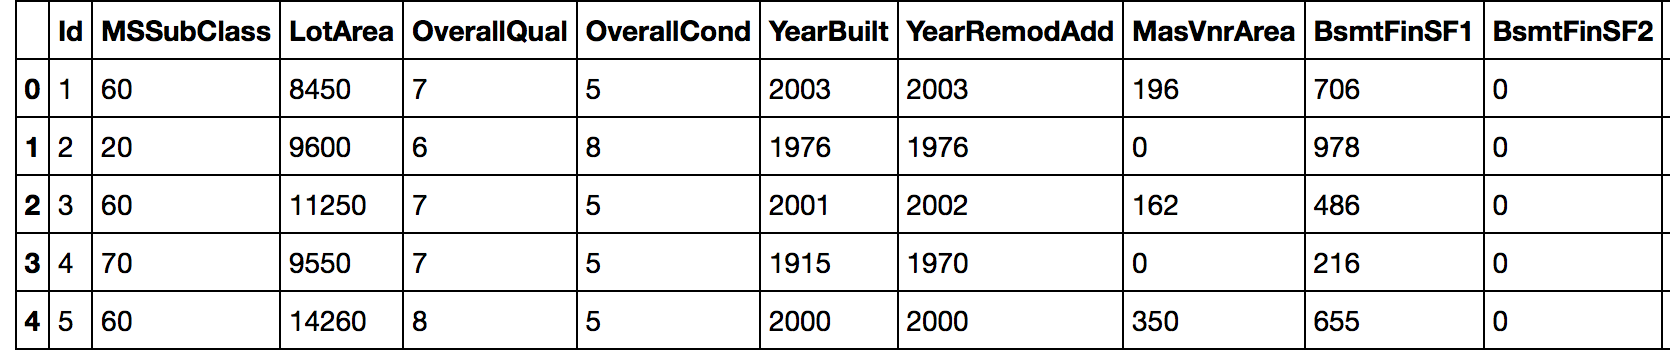
\includegraphics[width=0.95\columnwidth]{3}
\\
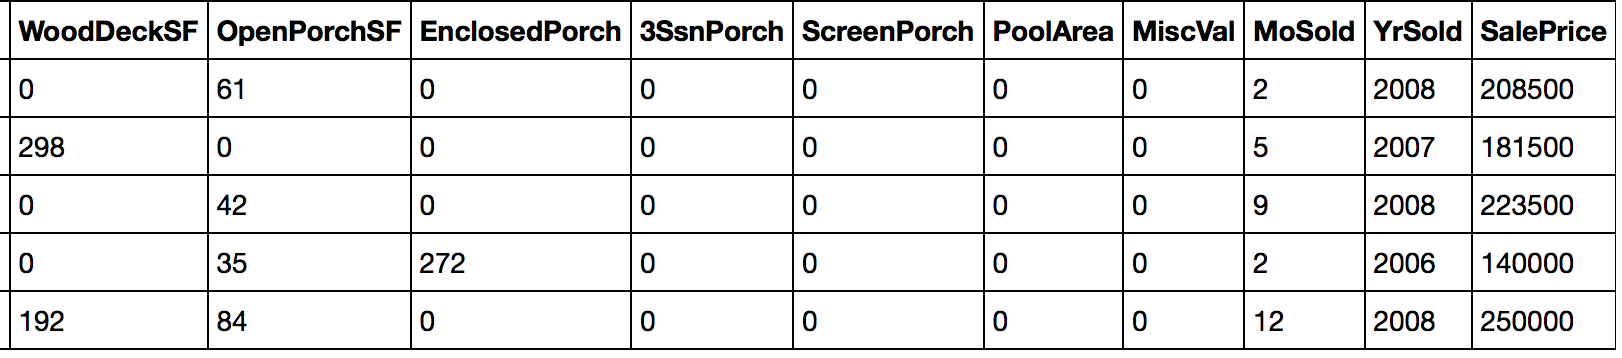
\includegraphics[width=0.95\columnwidth]{4}

\begin{lstlisting}
# clean data and show del df['error']
Out[26]:
df.head()

# clean data and show del df['error']
Out[26]:
df.head()
\end{lstlisting}
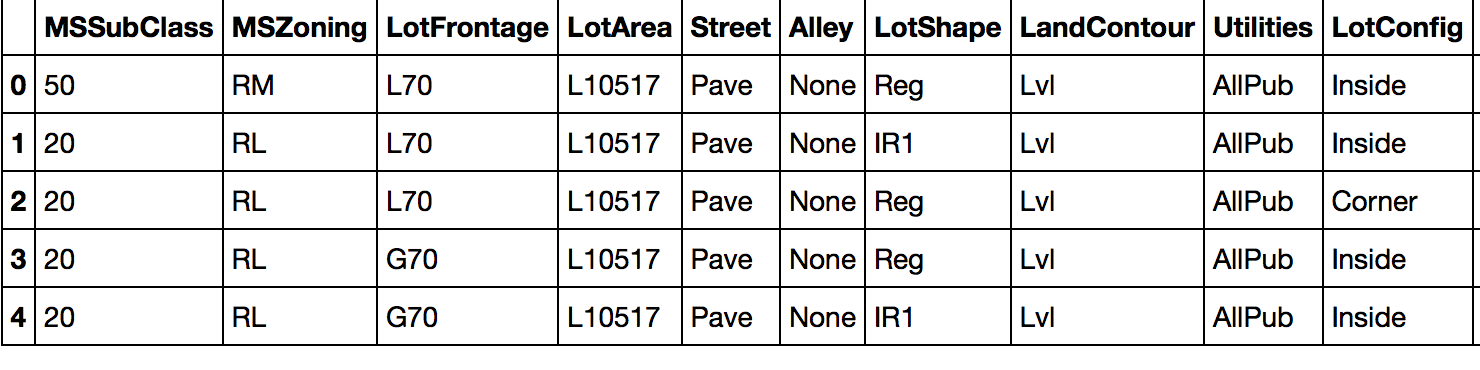
\includegraphics[width=0.95\columnwidth]{1}
\\
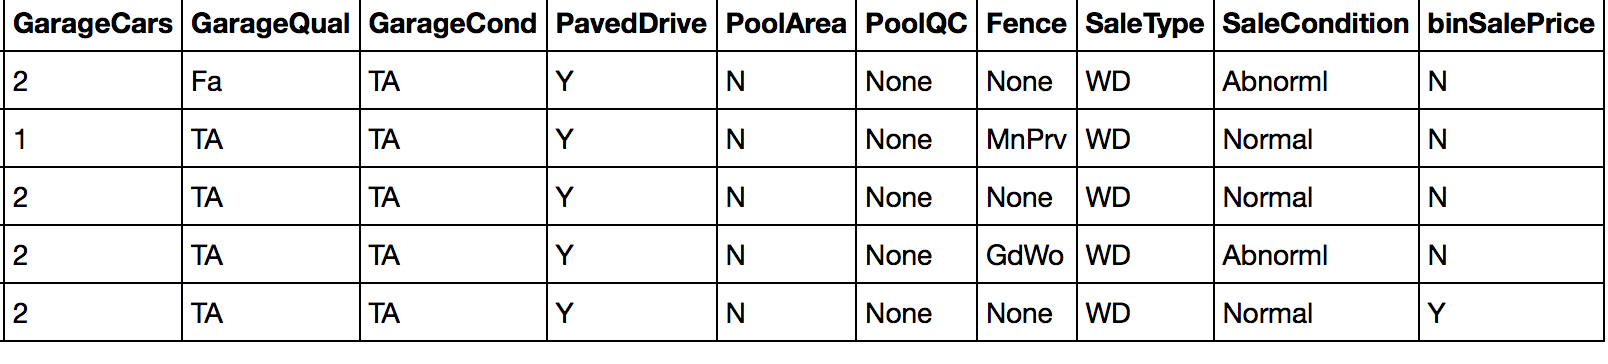
\includegraphics[width=0.95\columnwidth]{2}

\begin{lstlisting}
In [50]: # show the distribution of a column col = list(df['SalePrice'])
         plt.hist(col)
         plt.show()
         # show the distribution of another column
         col = list(df['MSSubClass'])
         plt.hist(col)
plt.show()
\end{lstlisting}

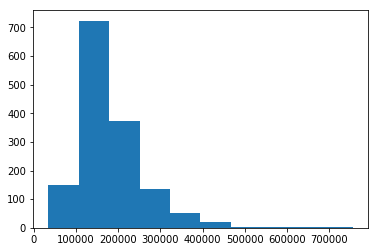
\includegraphics[width=0.95\columnwidth]{output_3_0.png}
\\
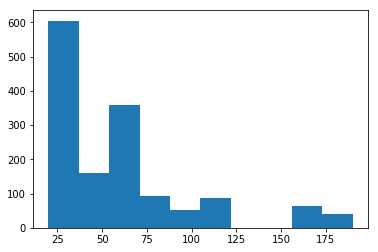
\includegraphics[width=0.95\columnwidth]{output_3_1.png}

\begin{lstlisting}
0.0.1 Splitting into train and test
In [6]: X = df[['MSSubClass','LotArea','OverallQual','OverallCond','YearBuilt', 'YearRemodAdd','
        y = df['SalePrice']
3
from sklearn.model_selection import train_test_split
        X_train, X_test, y_train, y_test = train_test_split(X, y, test_size=0.2, random_state=3)
In [7]: print("X_train: ")
        print(X_train.shape)
        print("y_train: ")
        print(y_train.shape)
        print("X_test: ")
        print(X_test.shape)
        print("y_test: ")
        print(y_test.shape)
\end{lstlisting}

\begin{lstlisting}
X_train:
(1168, 18)
y_train:
(1168,)
X_test:
(292, 18)
y_test:
(292,)
\end{lstlisting}

\begin{lstlisting}
0.0.2 Using Linear Regression
In [53]: # import model
from sklearn.linear_model import LinearRegression
         # instantiate
linreg = LinearRegression()
# fit the model to the training data (learn the coefficients)
         linreg.fit(X_train, y_train)
Out[53]: LinearRegression(copy_X=True, fit_intercept=True, n_jobs=1, normalize=False)


\end{lstlisting}


\begin{lstlisting}
0.0.3 show the coefficients of the linear regression model
In [54]: # print the intercept and coefficients print(linreg.intercept_)
print(linreg.coef_)
1624810.78299
[ -1.32598253e+02
   7.42385752e+01
   4.81195345e+00
1.17264859e+00
3.87166477e+02
3.94460800e+01
3.27974313e+04
6.87797648e+01
8.24586253e+01
3.52017131e+02
3.05508150e+01
2.55083195e+01
 3.67581004e+01   
 6.78306474e+01   
 1.90173648e+02 
 -2.30935682e+00
-7.58643734e+02  
-1.29045399e+03]
\end{lstlisting}

\begin{lstlisting}
In [57]: # pair the feature names with the coefficients list(zip(X, linreg.coef_))
Out[57]: [('MSSubClass', -132.59825288297418),
          ('LotArea', 1.1726485927894912),
          ('OverallQual', 32797.431340275551),
          ('OverallCond', 352.01713092259615),
          ('YearBuilt', 74.238575183515508),
          ('YearRemodAdd', 387.16647668821042),
          ('MasVnrArea', 68.779764836201025),
          ('BsmtFinSF1', 30.550814975040396),
          ('BsmtFinSF2', 4.811953445828749),
          ('WoodDeckSF', 39.446080031209931),
          ('OpenPorchSF', 82.458625258585016),
          ('EnclosedPorch', 25.508319545409904),
          ('3SsnPorch', 36.758100373945126),
          ('ScreenPorch', 67.830647415049953),
          ('PoolArea', 190.17364768682),
          ('MiscVal', -2.309356818373999),
          ('MoSold', -758.64373443570901),
          ('YrSold', -1290.4539903809468)]

\end{lstlisting}

\begin{lstlisting}
0.0.4 Make Prediction
In [58]: y_pred = linreg.predict(X_test)
         print(y_pred)
         [  93201.65287675  142554.76960023  207127.40186274  129212.10104713
  284603.13460876   65916.12615103  200722.35383783  169593.14341713
  138022.19789723  138387.20437863  143561.19507458  150824.4043784
  141397.06769187  242451.92943507  294242.12637714  155754.66681213
  137312.71913462  129724.80248527  114876.63835247  150591.3640421
  123366.39990094  150807.12337525  243530.22799299   80763.41783606
  197680.6442071   103336.1791911   164351.0638006    90905.30200621
  168564.67988019  115830.7939216   155494.23908365  100141.70869163
  129753.99108892  156909.62744952  198024.33401226  127554.26516619
  202396.44876193  110389.71894826  176051.07333227  145661.99691863
  220408.37444225  116538.72044784  244706.34275193  195197.31242857
  278775.03276079  152402.88891841  144044.1694957    99239.71058997
  131931.4514502   110682.0707577   286158.2247229   135834.2312254
   97216.99608222  143430.65499509  119919.1222882   142851.58478543
  204412.40936722  153442.22728046  132396.82935032  257628.30990488
  169933.91094914  120347.46703607  105703.73721332  334713.28117372
  114893.96280934  234743.60884166  183600.27577235  258490.04570492
  375690.10951031  111056.04841375  172340.59505253  136413.8949467
  144985.53609179  223770.11250678  153958.15058402  118182.70605492
  231712.95504903  102900.49898239  154389.2668046   127207.38840213
  145004.55720471  176843.72114247  169051.0221719   148482.89114126
5
313474.32652747  152493.90863482  173352.98469532  126431.410949
706997.59838104  273836.15113809  408289.15199464  184268.88377474
176636.23715661  275235.88756875  209025.79856597  301622.54866502
153471.41164935  210322.3456924   140373.14967059  147240.88073756
179983.14477495  236775.79874229  144459.66092891  253623.49760802
176613.8745506   229147.89622806  185611.33497853  184942.64455848
 68523.77301979  111428.57621911   95690.85464389  210924.92842256
236920.78986689  179625.99265486  146998.08010809  218710.14496723
128961.12389426  144822.81021683  180904.35339614  126176.27283423
 99200.6426002   257960.86042887  200015.00187306  189350.38765334
161309.58475033  188509.81215872  207842.304773    133745.60572444
146175.12018952  311506.70403465  123810.46022005  178891.00062911
161368.3460505   141225.57119693  247990.6084084   134197.93148368
105114.81700542   66238.30229136  178481.22924629  169327.77885027
115722.77661632  163980.78329632  259041.24033003  263441.73011914
283269.97449944  291907.40480834  197028.67375584  253486.2658659
104257.64311109  332402.81936497  235123.35447297  117530.28281743
331867.34936129  166007.48240655  203642.02685762  366937.27511738
254191.87188157  124456.0621068    91276.03127415  115556.73782587
135405.78846278  218110.30607514  214268.7945742   140032.81401882
182040.72686091  176083.82849172  189209.9335995   116292.72416312
156432.52235127  204191.85524977  243977.32691289  217247.92836948
285376.77266393  246843.94978091  222100.61618257  167537.81203899
173903.04681628  161022.49525822  142938.09421832  236955.86271045
118908.1141022   191184.99717802  264889.79476426  125154.14702448
227251.47377346  237911.61180972  161841.30235331  191446.14163809
116625.79736531  145735.12537565  105372.79335894  316582.43267848
122028.63732317  290593.52200424  185714.04747969  190352.49050499
231514.01368592  230079.79348368  127676.13717555  211300.51925447
195483.82714307  192652.60353829  165237.26624796  120930.29413027
246160.5957099   281456.29298689  246797.10864379  119311.41048692
125885.59543623  237312.78172775   80648.88617473  121685.26043487
114935.23554672  161184.27138098  148054.27442727  131650.06362918
201165.65733849  296531.91858395  130462.5135931   249027.70239568
177623.04403208  166277.96320103   94660.31809216   72766.55532673
120114.744019    102331.03622172  132734.52163217  195045.15386957
206238.5262443   254559.77871816  103180.37264793  217595.03298126
200740.09709761  309978.95599912  120679.0962053   105614.64472826
246644.91857921  132884.29067159  333136.91588735  167381.82062275
160037.46133837  280268.75854488  166764.14578859  163691.73116515
172120.87702276   86744.64311271  159726.64897898  152045.32160112
148376.7717957   261196.38354104  190853.69410498  147271.05605036
126117.61348537  122639.71249082  227607.46595295  170013.76929953
136917.40993332  157131.07140997  127090.52733891  135446.00011116
271380.56027395  138338.59566889  233995.26083728  141733.47586868
138265.15523182  200673.53942787  186815.23291077  226030.65231941
197560.45885543  392086.99980809  199746.97825355  194749.30417935
122346.88308178  170839.72571199   37264.46454778  153581.22281016
6
183230.11599231  143418.12876415  170655.31440413   60936.55821163
  279635.84539619  141986.8959917   163848.54119987  130962.64226048
  194210.12078339  222988.18563234  252212.98444331  371404.24966183
  219031.5941132    63288.51714085  112594.85348706  139413.4862122 ]
\end{lstlisting}

0.0.5 Finally Check Error
0.0.6 Here, we use Root Mean Squared Error (RMSE) which is the square root of the mean of the squared errors for error checking:
$$\sqrt{\frac 1n\sum_{i=1}^n(y_i-\hat{y}_i)^2}$$

\begin{lstlisting}
In [59]: from sklearn import metrics
         import numpy as np
         print(np.sqrt(metrics.mean_squared_error(y_test, y_pred)))
46554.0967726
\end{lstlisting}

\begin{lstlisting}
0.0.7 Using logistic Regression
In [8]: from sklearn.linear_model import LogisticRegression
        logreg = LogisticRegression()
        logreg.fit(X_train, y_train)
        y_pred = logreg.predict(X_test)
        print(y_pred)
\end{lstlisting}
\begin{lstlisting}
[135000 139400 215000  85000 259500 108480 161750  93000 103600 129500
  80000 112000 115000 194000 171000 145000 130250 130500 151000 395192
 135000 266500 335000 135000 197000 110000 116000 135000 139000  98000
 181000  52500 110000 161000 248328 149000 215000 112500 143000 138000
 224900  86000 215000 162900 190000 165500  79000  87000 135000 112000
 223000  85400  90000 145000 143000 129500 204900 145000 127500 275000
 194000 114500 157900 260400 143500 254900 180000 190000 223000 150000
 215000  89500 145000 276000 111250 220000 172500 118964 130500 127000
 137000 146000 196000 123600 380000 266500 229000 129900 324000 181000
 260400 144152 202500 279500 319000 190000 130500 167000 171000 140000
 142000 250000  98000 275000  79900 215000 193000 199900 139600 143000
 137450 185900 328900 215000 259500 205950  87000 143900 167240 127000
 101800 224900 196500 167000 108959 180000 162000 129900 176000 319000
 124500 155900 266000 106000 215000 147000 121600 110000 165000 176000
  79900 181000 195400 290000 315750 260400 153900 325624 112500 293077
 181000 141000 342643 139000 135000 325000 174000  82500  78000 131500
 120500 446261 378500 135000 191000 177500  79000  80000 258000 155900
 263000 220000 378500 165000 184900 214000 128500 165500 159000 185900
 160000 146000 240000 131500 328900 239000 166000 191000  80000 118000
  7
81000 325000 117500 222000 136905 202665 220000 266000 109500 244600
181000 159500 140000  98000 195400 184900 378500 110000 200000 278000
161500 135000 180500 144152 190000 114500 181134 297000 147000 143750
155900 142000 107500  99500 117500 116050 115000 181000 215000 203000
122000 138800 104900 315000 136905 169000 250000 149000 305900 149000
164900 229000 181000 158000 144000 125500 145000 243000 130500 250000
179900 158000 145000 117500 187500 145000 117000 130000 135000  99500
215000  89000 143000 189950 154000 145000 163000 200000 181000 264132
150000 289000 167000 137900  67000 145000 127500 141500 214000 151000
209500 118000 161500 127500 143250 230000 290000 485000 191000  85000
110000 173000]
\end{lstlisting}

\begin{lstlisting}
Classification accuracy: 
Proportion of correct predictions
Common evaluation metric for classification problems
In [10]: from sklearn import metrics
         import numpy as np
print(metrics.accuracy_score(y_test, y_pred))
0.0
\end{lstlisting}

\section{Algorithm Comparison and Analytics}
\par 
Linear Regression is used to establish a relationship between Dependent and Independent variables, which is useful in estimating the resultant dependent variable in case independent variable change. For example, using a Linear Regression, the relationship between Rain (R) and Umbrella Sales (U) is found to be - U = 2R + 5000. This equation says that for every 1mm of Rain, there is a demand for 5002 umbrellas. So, using Simple Regression, you can estimate the value of your variable.

\par 
Logistic Regression on the other hand is used to ascertain the probability of an event. And this event is captured in binary format, i.e. 0 or 1. For example, I want to ascertain if a customer will buy my product or not. For this, I would run a Logistic Regression on the (relevant) data and my dependent variable would be a binary variable (1=Yes; 0=No).

\par
In terms of graphical representation, Linear Regression gives a linear line as an output, once the values are plotted on the graph. Whereas, the logistic regression gives an S-shaped line

\par
The logistic model is unavoidable if it fits the data much better than the linear model. And sometimes it does. But in many situations the linear model fits just as well, or almost as well, as the logistic model. In fact, in many situations, the linear and logistic model give results that are practically indistinguishable except that the logistic estimates are harder to interpret.
\par
For the logistic model to fit better than the linear model, it must be the case that the log odds are a linear function of X, but the probability is not. And for that to be true, the relationship between the probability and the log odds must itself be nonlinear. But how nonlinear is the relationship between probability and log odds? If the probability is between .20 and .80, then the log odds are almost a linear function of the probability.

\par
Interpretability is not the only advantage of the linear probability model. Another advantage is computing speed. Fitting a logistic model is inherently slower because the model is fit by an iterative process of maximum likelihood. The slowness of logistic regression isn’t noticeable if you are fitting a simple model to a small or moderate-sized dataset. But if you are fitting a very complicated model or a very large data set, logistic regression can be frustratingly slow.

\par
The linear probability model is fast by comparison because it can be estimated noniteratively using ordinary least squares (OLS). OLS ignores the fact that the linear probability model is heteroskedastic with residual variance p(1-p), but the heteroscedasticity is minor if p is between .20 and .80, which is the situation where I recommend using the linear probability model at all. OLS estimates can be improved by using heteroscedasticity-consistent standard errors or weighted least squares. In my experience these improvements make little difference, but they are quick and reassuring.

\bibliographystyle{ACM-Reference-Format}
\bibliography{report} 

\end{document}



